
\documentclass{beamer}


\mode<presentation>
{
  \usetheme{Hawke}
  \setbeamercovered{transparent}
}


\usepackage[english]{babel}
\usepackage[latin1]{inputenc}
\usepackage{times}
\usepackage[T1]{fontenc}
\usepackage{multimedia}
\usepackage{mathtools}

%%%%%%
% My Commands
%%%%%%

\newcommand{\ml}{{\sc matlab}}
\newcommand{\bb}{{\boldsymbol{b}}}
\newcommand{\bx}{{\boldsymbol{x}}}
\newcommand{\bfm}[1]{{\boldsymbol{#1}}}

%%%%

\title[Lecture 2]{Lecture 2 - Linear Systems 1}
\author[I. Hawke]{I.~Hawke}
\institute[University of Southampton]
{
  School of Mathematics, \\
  University of Southampton, UK
}

\date[Semester 1] % (optional, should be abbreviation of conference name)
{MATH3018/6141, Semester 1}

\subject{Numerical methods}

\pgfdeclareimage[height=0.5cm]{university-logo}{mathematics_7469}
\logo{\pgfuseimage{university-logo}}

\AtBeginSection[]
{
  \begin{frame}<beamer>
    \frametitle{Outline}
    \tableofcontents[currentsection]
  \end{frame}
}


\begin{document}

\begin{frame}
  \titlepage
\end{frame}

\section{Linear systems}

\subsection{Reminders}

\begin{frame}
  \frametitle{Revisions and reminders}

  The system of linear equations
  \begin{equation*}
    \left\{
      \begin{aligned}
          x +   y & = 1 \\
        2 x + 2 y & = 3
      \end{aligned}
    \right.
  \end{equation*}
  has no solutions; the system
  \begin{equation*}
    \left\{
      \begin{aligned}
        0.9999999  x +   y & = 0.9999999 \\
        2          x + 2 y & = 2.9999999
      \end{aligned}
    \right.
  \end{equation*}
  does. \pause

  In general form
  \begin{equation*}
    A \bx = \bb
  \end{equation*}
  has a unique solution iff $\det (A) \ne 0$.

\note{
 Written in the general form
  \begin{equation*}
    A \bx = \bb
  \end{equation*}
  with $A$ an $n \times n$ matrix, we know that the system has a
  unique solution iff $\det (A) \ne 0$.
}

\end{frame}


\subsection{Aim}

\begin{frame}
  \frametitle{Aim of condition number}

  The two systems
  \begin{equation*}
    \left\{
      \begin{aligned}
          x +   y & = 1 \\
        2 x + 2 y & = 3
      \end{aligned}
    \right., \quad
    \left\{
      \begin{aligned}
        0.9999999  x +   y & = 0.9999999 \\
        2          x + 2 y & = 2.9999999
      \end{aligned}
    \right.
  \end{equation*}
  are indistinguishable at 6-digit precision; such a ``computer''
  cannot tell if \emph{either} system has a well-defined solution!
  \pause

  \vspace{1ex}

  Systems are \emph{ill-conditioned}: a ``small'' input change leads
  to an enormous change in the solution. \pause The \emph{condition
    number} should predict ill-conditioned systems without finding
  solutions first. \pause

  \vspace{1ex}

  Note: as the very notion of ``small'' depends on the precision, so
  must the interpretation of the condition number.

\end{frame}

\subsection{Options}

\begin{frame}
  \frametitle{Determinants}

  Think about the determinant $\det(A)$. If it vanishes there is no
  solution. \pause

  \vspace{1ex}

  But the matrix
  \begin{equation*}
    A = 10^{-1}
    \begin{pmatrix}
      1 & 0 & \dots & 0 \\
      0 & 1 & \ddots & \vdots \\
      \vdots & \ddots & \ddots & 0 \\
      0 & \dots & 0 & 1
    \end{pmatrix}
  \end{equation*}
  has determinant $10^{-n}$: arbitrarily small, whilst the matrix is
  trivial to invert.

  \vspace{1ex}

  Determinant $\ne$ condition number.

\end{frame}

\begin{frame}
  \frametitle{Perturbations}

  Model the effect of errors by using a parameter $\epsilon$:
  $\epsilon = 0$ means the exact solution. We write
  \begin{equation*}
    \left( A + \epsilon F \right) \bx (\epsilon) = \bb.
  \end{equation*}
  %
  \begin{center}
    \includegraphics<1|handout:0>[width=0.7\textwidth]{figures/Perturbations}
  \end{center}
  %
  \pause
  %
  Differentiate wrt $\epsilon$ giving $A \dot{\bx} = - F \bx + {\cal
    O}(\epsilon)$ and Taylor expand to find
  \begin{equation*}
    \bx(\epsilon) - \underbrace{\bx(0)}_{\smash{\text{exact}}} =
    \epsilon \dot{\bx}(0) + {\cal O}\left( \epsilon^2 \right) = -
    \epsilon A^{-1}  F \bx + {\cal O}\left( \epsilon^2 \right).
  \end{equation*} \pause
  %
  To get a \emph{relative} error we need a magnitude or absolute
  value, giving
  \begin{equation*}
    \frac{\| \bx(\epsilon) - \bx \|}{\| \bx \|} \sim \| A^{-1} \| \| A
    \| \left( \epsilon \frac{\|F\|}{\|A\|} \right).
  \end{equation*} \pause
  The part we can measure is the \emph{condition number}
  $K(A) = \| A \| \| A^{-1} \|$.

\end{frame}

\subsection{Vector norms}

 \begin{frame}
   \frametitle{Vector norms}

   Norms are ``mathematical distance functions''. Focus on real
   vectors, e.g.\ to find the error $\| \bx_{\text{num}} -
   \bx_{\text{exact}} \|$. Interesting norms are
   \begin{equation*}
     \| \bx \|_1 \equiv \sum_{j=1}^n | x_j |, \quad
     \| \bx \|_2 \equiv \left[ \sum_{j=1}^n ( x_j )^2 \right]^{1/2}, \quad
     \| \bx \|_{\infty} \equiv \max_j | x_j |.
   \end{equation*} \pause

   {\bf Example}: If $\bx = (-1, 2, 1)$ then
   \begin{align*}
     \| \bx \|_1 & = | -1 | + | 2 | + | 1| &&= 4, \\
     \| \bx \|_2 & = \sqrt{(-1)^2 + (2)^2 + (1)^2} &&= \sqrt{6}, \\
     \| \bx \|_{\infty} & = \max (| -1 |, | 2 |, | 1 |) && = 2.
   \end{align*}

   \note{
   Norms are ``mathematical distance functions''; they impose a
   structure on a mathematical space describing the separation of
   points in that space. The norms above are examples of $p$-norms on
   a simple space. In general norms obey simple properties like
   linearity, positivity, and the triangle inequality.
   }

 \end{frame}

 \begin{frame}
   \frametitle{Vector norms - geometrically}

   \begin{center}
     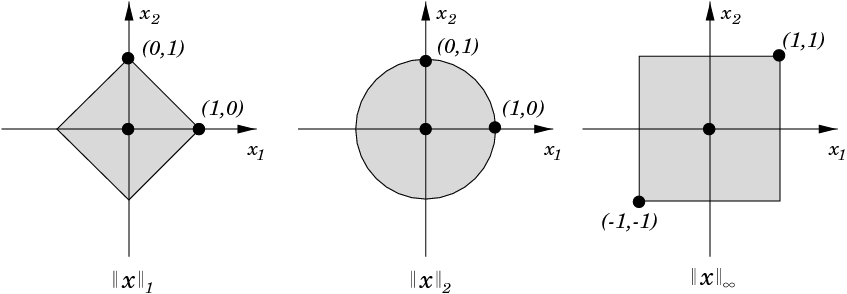
\includegraphics[width=0.9\textwidth]{figures/norms}
   \end{center}
   By plotting the region of $\mathbb{R}^2$ defined by $\| \bx \| \le
   1$ we see the different geometric meanings of the norms.

 \end{frame}


 \subsection{Matrix norms}

 \begin{frame}
   \frametitle{Matrix norms}

   Our suggested condition number $K(A) = \| A \| \| A^{-1} \|$ needs
   a \emph{matrix}, not vector norm.

   \vspace{1ex}

   Induce a norm with respect to a vector: If $\bfm{y}$ is a vector
   then $A\bfm{y}$ is also a vector, so we can use a vector
   norm. \pause

   \vspace{1ex}

   To get a \emph{representative, finite} answer we use
   \begin{equation*}
     \| A \| = \max_{\| \bfm{y} \| = 1} \| A \bfm{y} \|.
   \end{equation*}

   \vspace{1ex}

   {\bf Remark}: All the norms used in the above \emph{must} be the
   same.

   \note{
   The vector norms above are a good way of quantifying the difference
   between known solutions, such as the computed solution and the true
   solution. However, we want a prediction \emph{without} computation
   of how good we expect the solution to be. To do this we need to
   extend to matrix norms.
   }

 \end{frame}

 \begin{frame}
   \frametitle{Examples of matrix norms - 1 norm}

   The matrix 1-norm reduces to the maximum of the 1-norms of the
   column vectors of $A$. \pause

   Let
   \begin{equation*}
     A =
     \begin{pmatrix}
       1 & 2 & 3 \\
       4 & 5 & 4 \\
       -1 & 0 & 2
     \end{pmatrix}.
   \end{equation*} \pause
   The column vectors are
   \begin{equation*}
     \bfm{c}_1 =
     \begin{pmatrix}
       1 \\ 4 \\ -1
     \end{pmatrix}, \quad
     \bfm{c}_2 =
     \begin{pmatrix}
       2 \\ 5 \\ 0
     \end{pmatrix}, \quad
     \bfm{c}_3 =
     \begin{pmatrix}
       3 \\ 4 \\ 2
     \end{pmatrix}.
   \end{equation*} \pause
   The resulting 1-norms are
   \begin{equation*}
     \| \bfm{c}_1 \|_1 = 6, \quad
     \| \bfm{c}_2 \|_1 = 7, \quad
     \| \bfm{c}_3 \|_1 = 9.
   \end{equation*} \pause
   Therefore the 1-norm of $A$ is
   \begin{equation*}
     \| A \|_1 = \max ( \| \bfm{c}_1 \|_1, \| \bfm{c}_2 \|_1, \| \bfm{c}_3
     \|_1 ) = 9.
   \end{equation*}
 \end{frame}

 \begin{frame}
   \frametitle{Examples of matrix norms - $\infty$ norm}

   The matrix infinity-norm reduces to the maximum of the 1-norms of
   the row vectors of $A$. \pause

   Let
   \begin{equation*}
     A =
     \begin{pmatrix}
       1 & 2 & 3 \\
       4 & 5 & 4 \\
       -1 & 0 & 2
     \end{pmatrix}
   \end{equation*}
   as before. \pause The  vectors are
   \begin{equation*}
     \bfm{r}_1 =
     \begin{pmatrix}
       1 & 2 & 3
     \end{pmatrix}, \quad
     \bfm{r}_2 =
     \begin{pmatrix}
       4 & 5 & 4
     \end{pmatrix}, \quad
     \bfm{r}_3 =
     \begin{pmatrix}
       -1 & 0 & 2
     \end{pmatrix}.
   \end{equation*} \pause
   The resulting 1-norms are
   \begin{equation*}
     \| \bfm{r}_1 \|_1 = 6, \quad
     \| \bfm{r}_2 \|_1 = 13, \quad
     \| \bfm{r}_3 \|_1 = 3.
   \end{equation*} \pause
   Therefore the $\infty$-norm of $A$ is
   \begin{equation*}
     \| A \|_{\infty} = \max ( \| \bfm{r}_1 \|_1, \| \bfm{r}_2 \|_1, \| \bfm{r}_3
     \|_1 ) = 13.
   \end{equation*}

 \end{frame}


 \subsection{The condition number}

 \begin{frame}
   \frametitle{The condition number}

   Define the condition number as
   \begin{equation*}
     K(A) = \| A \| \| A^{-1} \|.
   \end{equation*}
   Any norm can be used, but for simplicity the 1- or $\infty$-norms
   are usual. \pause

   \begin{overlayarea}{\textwidth}{0.5\textheight}
     \only<2>
     {
       Loose interpretation: the condition number is
       \emph{the amount that inverting the matrix will increase any
         intrinsic error in the coefficients}.
     }
     \only<3->
     {
       More strictly, define the \emph{weighted residual} as
       \begin{equation*}
         {\cal E} = \frac{\| A \bx_{\text{num}} - \bb \|}{\| \bb \|}.
       \end{equation*}
       This can be minimized numerically. \pause It can be shown that:
       \begin{equation*}
         \frac{1}{K(A)} {\cal E} \le \frac{ \| \bx_{\text{num}} -
           \bx_{\text{exact}} \|}{\| \bx_{\text{exact}} \|} \le  K(A)
         {\cal E} .
       \end{equation*}
       Controlling ${\cal E}$ does not control relative error if $K(A)
       \gg 1$!
     }
   \end{overlayarea}

 \end{frame}

 \begin{frame}
   \frametitle{Condition number example}

   Consider the matrix
   \begin{equation*}
     A =
     \begin{pmatrix}
       1 & 2 \\
       \tfrac{499}{1000} & \tfrac{1001}{1000}
     \end{pmatrix}.
   \end{equation*} \pause
   The inverse is
   \begin{equation*}
     A^{-1} =
     \begin{pmatrix}
       \tfrac{1001}{3} & -\tfrac{2000}{3}  \\
       -\tfrac{499}{3} & \tfrac{1000}{3}
     \end{pmatrix}.
   \end{equation*} \pause
   The matrix norms are
   \begin{align*}
     \| A \|_1 & = 3.001, & \| A^{-1} \|_1 & = 1000 \\
     \| A \|_{\infty} & = 3, & \| A^{-1} \|_{\infty} & = 1000
     \tfrac{1}{3}.
   \end{align*} \pause
   Hence the condition number is $K(A) = 3001$. We should expect that
   if the coefficients of the matrix are uncertain in the third
   significant figure then the result of solving a linear system with
   this coefficient matrix will be uncertain to ${\cal O}(1)$ (see
   course notes).

 \end{frame}


 \section{Summary}

 \subsection{Summary}

 \begin{frame}
   \frametitle{Summary}

   \begin{itemize}
   \item Linear systems where a ``small'' change in the coefficients
     means a large change in the solution are called
     \emph{ill-conditioned}.
   \item The \emph{condition number} $K(A) = \| A \| \| A^{-1} \|$
     gives a measure for any given matrix without having to compute
     the solutions.
   \item Whether a condition number is ``too large'' or not depends on
     the precision to which you are working and the accuracy with
     which the coefficients are known.
   \item The condition number depends on matrix norms; for simplicity
     we only consider simple matrix norms induced by standard vector
     norms.
   \item The condition number can be approximated rapidly
     \emph{without} inverting the matrix; this makes it useful as an
     pre-check.
   \end{itemize}

 \end{frame}



\end{document}



%%% Local Variables:
%%% mode: latex
%%% TeX-master: t
%%% End:
